% !TEX root = ../thesis-example.tex
%
\chapter{Related Literature}
\label{sec:related}
Algorithmic trading (hereafter, referred to as AT) has been present since the mid 1990s with the rise of personal computer power and the internet \cite{WEB:PISANI:2010}. Documenting these methods towards the volatile and unregulated market of cryptocurrency (hereafter, referred to as crypto) will address the little related literature present due to the infancy of crypto markets. This project hopes to address this gap by applying tested methods used on the stock and currency market, while building a platform to utilise the bot. This chapter will discuss the topics Algorithmic Trading, Trading Indicators And How Strategies Use Them, and Crypto And Their Markets. These topics will provide an understanding of how algorithms are used and why they have become a necessity for the operation of the stock market. Illustrating how these trading methods work will show why they can also be applied to crypto. I will also cover varying types of trading indicators used in strategies, show how effective they are and why they would be useful towards AT in crypto. Finally, I will introduce the world of crypto and how their markets operate. I will discuss what makes the crypto market unique, compare against the tested stock market and explain how using the aforementioned trading methods can allow for it to be exploited. 
% \cleanchapterquote{A picture is worth a thousand words. An interface is worth a thousand pictures.}{Ben Shneiderman}{(Professor for Computer Science)}


\section{Algorithmic Trading}
\label{sec:related:algoTrading}
\noindent Treleaven, Falas and Lalchand \cite{ART:Treleaven:2013} defines AT as "any form of trading using sophisticated algorithms (programmed systems) to automate all or some part of the trade cycle". AT fits into systematic trading, described as trading based on rules. This combines both trend analysis (slow, discussed in section \ref{sec:related:algoTrading:tradeprocess}) and high-frequency (fast, discussed in section \ref{sec:related:algoTrading:HFT}) trading. Nuti, Mirghaemi, Treleaven (who is also in \cite{ART:Treleaven:2013}) and Yingsaeree \cite{ART:Nuti:2011} state AT was designed to automate trade while being profitable and executing orders optimally. These characteristics of AT have allowed it to fit into a wide range of use cases, which is why it is so widely used on equity markets, resulting in 90 percent of the total daily trade volume in the EU and US markets today \cite{WEB:Cheng:2017,ART:Kolakowski:2018}. The computational power and accuracy of AT demonstrates as to why this is the case and is seen through my discussions on the process of how trades come to fruition. Illustrating how these steps are taken demonstrate what this project can expect to implement.

\subsection{Trade Process}
\label{sec:related:algoTrading:tradeprocess}
The trade process for AT described by Nuti et al \cite{ART:Nuti:2011} and Treleaven et al  \cite{ART:Treleaven:2013} consists of data access, pre-trade analysis, trading signal generation, trade execution, and post-trade analysis. The listed steps (figure \ref{fig:related:tradeprocess}) define key actions required to analyse data to determine if the market conditions can turn a profit in the entry or exit of an asset. The ultimate goal of AT is to gain profit or know when to cut losses, where Nuti et al \cite{ART:Nuti:2011} and Treleaven et al  \cite{ART:Treleaven:2013} agree are addressed by these steps. The research of this trading process capture the fundamental variables required for an algorithm to work, considering all aspects of the market to trade on.

\begin{figure}[htb]
    \centering
	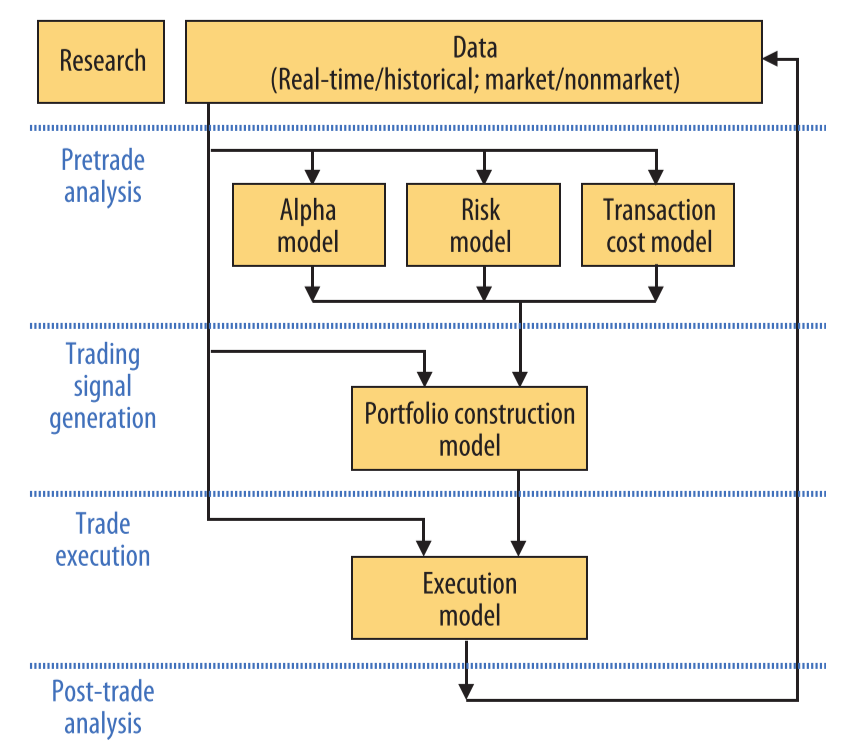
\includegraphics[width=0.55\textwidth]{content/graphics/AT-trade_process}
	\caption{Trade Process Figure by Nuti et al \cite{ART:Nuti:2011}: \textit{(a)} Research / Data, \textit{(b)} Pre-trade Analysis, \textit{(c)} Trading Signal Generation; \textit{(d)} Trade Execution, \textit{(e)} Post-trade Analysis }
	\label{fig:related:tradeprocess}
\end{figure}

Treleaven et al \cite{ART:Treleaven:2013} discuss that access to clean data is crucial to the operation of AT. The specificity of data required depends on the type of algorithm being built. Treleaven et al describe data which can vary from financial, economic, social and news to real-time, historic and analysed market data. The selection and validity of data can greatly affect the operation of AT and requires vetting of cleanliness. This is consistent with Chan's \cite{BOOK:Chan:2013}  discussion of using data to simulate strategies using backtesting, where the results of a strategy may appear positive, but performs poorly when applied to out-sample real-time data. This suggests that the data used in backtesting may be limited, failing to cover the scope of the market. Considering this, implementing a robust system on backtesting that covers various different data sets would ensure the algorithm prevents unforeseen issues.

Both Treleaven et al \cite{ART:Treleaven:2013} and Nuti et al \cite{ART:Nuti:2011} describe that pre-trade analysis discerns trading opportunities from data with the aim of predicting future prices to generate trading signals. Specifics of how this is achieved is discussed in section \ref{sec:related:tradingStrategies}, but the three main categories of analysis are fundamental\footnote{Information relating to markets to determine an asset's fair value e.g. interest rates}, technical\footnote{Historic, current, and other market information to predict future prices} and quantitative\footnote{Mathematical models based on treating assets prices as random rather than deterministic (like technical analysis)}. As technical analysis is the aim of this project, the forecast of prices and momentum are based on trend indicators and other market data. Three mathematical models: alpha, risk and transaction cost (figure \ref{fig:related:tradeprocess}, part b) are used to predict future behaviour, evaluate levels of risk and determine potential costs induced respectively. Each model is crucial to determine the success rate of the entry into - or exit from - the market, but I would emphasise that the risk model may be the most crucial. Taking precautions to ensure risk is minimised is one of the biggest factors to ensure profitable trades, concluded by Engle, Ferstenberg and Russel \cite{ART:Robert:2012} that majority of traders opt for strategies that are risk averse.

Trading signal generation differs from pretrade analysis, specifically determining the values the trade should execute with. Here is why AT positions 90 percent of daily trade volume \cite{WEB:Cheng:2017,ART:Kolakowski:2018} with its ability to analyse all market information in milliseconds, allowing it to find the entry points with minimal risk. Nuti et al \cite{ART:Nuti:2011} define two problems that could occur during entry, oscillating buy and sell signals and incorrect model assumptions.  Kaufman \cite{BOOK:Kaufman:2013} discusses indicators (see section \ref{sec:related:tradingStrategies}) that can be unprofitable if oscillating prices are failed to be addressed. High transaction costs and increased losses can occur as a result of this. Detecting when to exit by taking profits or minimising losses is crucial, so by failing to address both of these points could lead to an unprofitable and useless signal. 


Finally, Nuti et al \cite{ART:Nuti:2011} and Treleaven et al \cite{ART:Treleaven:2013} states that trade execution determines the constraints a transaction can occur, such as costs or duration. The main point made at this stage is to not adversely affect the market with large orders, while executing trades with reduced risk. Deciding whether to split large orders up into smaller chunks could prevent a change of market momentum, but the time to fill your order results in obtaining a good price. Considering this, research by Engle et al \cite{ART:Robert:2012} states there is a risk component involved in time taken to execute a transaction. The low liquidity and high volatility of the crypto market would bolsters this risk factor, requiring extra attention to trade executions. 


For example, a market order\footnote{Buying/Selling an asset at the best possible price at the current time} during low liquidity would most likely result in overpaying for an asset and increasing volatility, whereas by placing a limit order\footnote{Buying/Selling an asset for a set price} can allow for a better price to fill over a longer period. However, this can also produce issues such as being cut above by a higher placed limit order, reducing the chances of your order filling at the quoted price. Continued analysis even after a trade has executed is required to minimise risk until the order is filled.

The trading process described by Nuti et al \cite{ART:Nuti:2011} and Treleaven et al \cite{ART:Treleaven:2013} correlates with how an algorithmic trading bot to crypto could be implemented. Using the aforementioned process determines steps at the pre-trade analysis stage to minimise risk while considering how to actually execute the trade. Demonstrating research and discussing common pitfalls of these stages shows how a well-designed trading bot can be implemented using technical analysis. While the trade process is discussed, not much about the actual implementation or success of these systems is mentioned. Taking factors such as risk based on transaction times and costs, and generating trade signals on correct analysis provides steps this project will follow. This paper will also discuss how these steps can be applied to the nascent crypto market, using real data and providing results based on analytics. Although this project looks to build a trading bot based on a form of slower pre-trade analysis, High-Frequency Trading constitutes the bulk of AT used in the stock market today. 

\subsection{High Frequency Trading}
\label{sec:related:algoTrading:HFT}
\noindent  Seth \cite{WEB:SETH:0001} states the largest category of the AT cohort is associated to High-Frequency Trading (hereafter, referred to as HFT). While low latency HFT is not possible in the crypto market (see section \ref{sec:related:cryptoAndTheirMarkets}) - and not used in the development of this project - discussing the effects that HFT has on the stock market is beneficial to evaluating its health and what the crypto market can expect. HFT is the primary trading type in the modern stock market characterised by the speed and volume of trades it can execute within a small-time frame.

Both Seth \cite{WEB:SETH:0001} and Chorida, Goyal, Lehmann and Saar \cite{REPORT:ChordiaEtAl:2013} state the fundamental requirement for a successful HFT algorithm is low latency - defined by Chorida et al as "strategies that respond to market events in the millisecond environment". This is evident by trading firms spending substantial amounts to be placed as close as possible to the exchange's server to remove milliseconds off latency times \cite{ART:Aswani:2016}. This allows trading firms to respond to the most recent market data, providing the advantage to the first trader that receives the data. Comparing human ability to analyse and respond in this time-frame displays why HFT is the primary method to transact on the market.

Chorida et al \cite{REPORT:ChordiaEtAl:2013} state that most of the liquidity in the stock market is provided by HFT algorithms based on their identifiable activities. This appears inline with an article by Warmbrodt \cite{ART:Warmbrodt:2016}, however he hinges on this as a defence traders use towards the uncertainty regulators face with volatility from events like the 2010 ``flash crash''. He also explains that Clinton had plans for a financial reform to tax certain types of harmful HFT in her presidential race. This reform would of reduced the profitability of HFT, resulting in less firms using this method which may of potentially hindered market quality. Events like the ``flash crash'' shows the extent of controversy that HFT is facing, with Nuti et al \cite{ART:Nuti:2011} and Treleaven et al \cite{ART:Treleaven:2013} basing this on the lack of knowledge towards how they operate. Warmbrodt \cite{ART:Warmbrodt:2016} discusses the findings from an investigation, calling this `predatory' behaviour from aggressive AT firms. 

However, other officials outline the positives of HFT with Warmbrodt \cite{ART:Warmbrodt:2016} quoting the US `Securities and Exchange Commission' (SEC) Chairwoman stating, "[investors] are doing better in today's algorithmic marketplace than they did in the old manual markets". Warmbrodt adds that this is apparent to lower trade costs present in today's markets. The increased liquidity HFT brings allows for larger orders to be successful close to the current price and execute within a short period.  Bajpai \cite{WEB:Bajpai:0001} builds on this by stating that "liquidity is an important characteristic of a good market". The price difference between the highest buy order and the lowest sell order, also known as the `bid-ask spread', reduces transaction costs by producing smaller differences between the buy and sell prices. This incentivises multiple orders to be made consistently by traders, with little transactional cost. In turn, the market is provided with liquidity which ultimately reduces risk for investors. Whether the effects of HFT on the market is resulted by poor understanding or some exploitative behaviour, further research is required to allow regulators to put protective measures in place. 

While Chorida et al \cite{REPORT:ChordiaEtAl:2013} agrees that when HFT operates correctly it can improve the quality of the market with liquidity, it can also degrade it by demanding liquidity without any market makers to fill this demand. This subsequently increases volatility by occurring a major shift in the assets price. Chorida et al state this is evident by the ``flash crash`` of May 2010 where HFT - while it may not of triggered it - certainly affected price volatility. As most HFT algorithms follow trends, they tend to trade on similar rules. An article by Kolakowski \cite{ART:Kolakowski:2018} describes this as `herd' behaviour on steroids, quoting the director of Exchange-Traded Fund (ETF), "when selling happens, more selling can occur and when buying happens, more buying can occur". This can pull liquidity from the market allowing the price to tumble, especially when AT controls roughly $8.8 trillion according to a 2016 study\cite{ART:Kolakowski:2018}. 

A source from Anagnostidis \cite{UNPUB:Anagnostidis:2017} explains "the speed with which the quotes are posted and cancelled has been criticised by market participants because its creates a false sense of deep liquidity supply for a stock". While this seems to counter previous points of HFT supplying liquidity, it's important to emphasise this is referring to \textit{deep} liquidity. It is undeniable that HFT provides vast amounts of liquidity as mentioned above. Anagnostidis summarises by stating that liquidity generated by submissions and cancellations does not translate into a persistent effect on liquidity supply. This false cushion of liquidity is derived by the current rules followed HFT algorithms and their herd like behaviour as discussed by Kolakowski \cite{ART:Kolakowski:2018}. This can greatly impact the stability of the market as a whole and is the main source for concern about HFT's affect to regulators \cite{WEB:Kaufman:2016}.   

However, this method of `submit-cancel` is also used for price discovery\footnote{Determining price of asset based on analysis of buyer and sellers} of an asset due to AT's precise market analysis. It provides informative predictions based on all market information available leading to readjustment of order prices. An empirical study by Brogaard, Hendershott and Riordan \cite{UNPUB:Brogaard:2017} concluded that HFT improves pricing efficiency\footnote{The assets price is best reflected by all information possessed} by "trading in the price's permanent direction and against transitory pricing errors". This is inline with another empirical study by Benos and Sagade \cite{ART:BENOS:2016} stating non-passive HFT flows in the direction of future price changes. It becomes apparent that price discovery and efficiency is improved by HFT as they tend to follow market trends.  

HFT is possible in the crypto markets but not to the same extent as the equity market. The lack of low latency connections partially prevents the evident positive and negative effects described above. While tightening spreads, reducing transaction costs, improving price discovery and strengthening price efficiency would contribute to the market's health overall, it is still in an unknown area of regulation to prevent negative damage. This leaves low latency HFT producing damaging effects with the described `herd' mentality contributing to the rise of flash crashes.  However, with the crypto market still being unregulated with extreme volatility, perhaps employing low latency HFT could still improve upon the current market's quality. Ultimately, the adverse effects are resulted by the domination of AT in the equity market over many years of development. Perhaps by the time crypto establishes and grows it's market, better regulation for itself and HFT could be further developed.



\section{Trading Strategies}
\label{sec:related:tradingStrategies}
\noindent As discussed in the trade process (See section \ref{sec:related:algoTrading:tradeprocess}), a well defined trading strategy is the basis of pre-trade analysis. Lien \cite{BOOK:Lien:2016} states that technical analysis works well in the fiat currency\footnote{Legal tender which does not have intrinsic value but declared to have value by the government} market due to its speculative nature and its tendency to overshoot and correct. Applying the indicators Lien discusses will define market trends in the crypto market, providing market interpretation for this project and the construction of a sound strategy. A paper from Detzel, Liu, Stauss, Zhou and Zhu \cite{ART:DetzelEtAl:2018} concluded through their use of technical analysis that they were able to predict returns on Bitcoin through use of moving averages on in-sample and out-sample data. This shows promising results towards the scope of this project, suggesting that technical analysis can effectively be applied to real-time market information. The moving averages indicator discussed by Detzel et al \cite{ART:DetzelEtAl:2018} and Lien \cite{BOOK:Lien:2016} provide clear trends and will be one of the main focuses towards this project. I will also look at relative strength index (RSI) and moving average convergence/divergence (MACD) momentum indicators and discuss their beneficial uses toward analysis of market trends.

A moving average (MA) is the mean of closing prices on intervals over a defined period - e.g. 12 days - and is described by Kaufman \cite{BOOK:Kaufman:2013} to remove market noise and find the direction of the price. The most common MA is the simple MA (SMA). Kaufman \cite{BOOK:Kaufman:2013} states that SMA can have abrupt changes in value when a significant price movement is dropped off the end. While this could be an issue in the fiat currency market, crypto markets are extremely volatile and are mostly based on significant news and biased trading rather than fundamental values, as discussed in section \ref{sec:related:cryptoAndTheirMarkets}, incurring significant price movements frequently. By dropping off these apparent "random" price jumps may potentially show a more accurate price. 

However, more responsive MAs may suit the crypto market such as the exponential moving average (EMA) suggested by Kaufman \cite{BOOK:Kaufman:2013}, being summarised to give greater weighting to more recent prices. Thus, the effect of dropping off the end price is reduced. The comparison on effectiveness of both of these MAs is a missing discussion by both Kaufman \cite{BOOK:Kaufman:2013} and Lien \cite{BOOK:Lien:2016}, but it is worth noting that EMAs are used frequently in other indicators, as I discuss later in this section. This would suggest an improved effectiveness compared to SMA at accurately predicting the trend in the current market price. Harmon \cite{BOOK:Harmon:2014} suggests that using a smaller time-frame with SMA than using an EMA could provide similar results, although, he presents no justification or acknowledgement to the SMA drop-off issue and seems to be merited on opinion. 
    
While SMA can be responsive to the current market price, the weighting of previous prices being equivalent to the current price results in a smooth trend line indicator. Whereas, EMA responds quicker to the current market price, but due to lower weighting of older prices results in a more jagged trend line. I lean more towards EMA to give the best insight towards market trends due to the volatility of crypto's market conditions and hence the need to react to these price changes quickly. Harmon \cite{BOOK:Harmon:2014} also states that EMAs are consistently used throughout other indicators with traders converting to EMA. However, the use, analysis, and comparison of both MAs in this project will be beneficial to draw conclusions as to which is more effective towards crypto.

Kaufman \cite{BOOK:Kaufman:2013} describes that the RSI indicates when overbought or oversold conditions occur. This is determined by dividing the total upward price changes over the total downward price changes from a period of time, and then fitted into a range of 0 to 100. This gives the measurement of the current price movement's relative strength of the defined period. This indicator will help determine if a trend reversal is likely to happen based on exceeding or dipping below the threshold values 70 and 30 respectively. Lien \cite{BOOK:Lien:2016} illustrates an example of using RSI identify when to enter the market. 

\begin{figure}[htb]
    \centering
	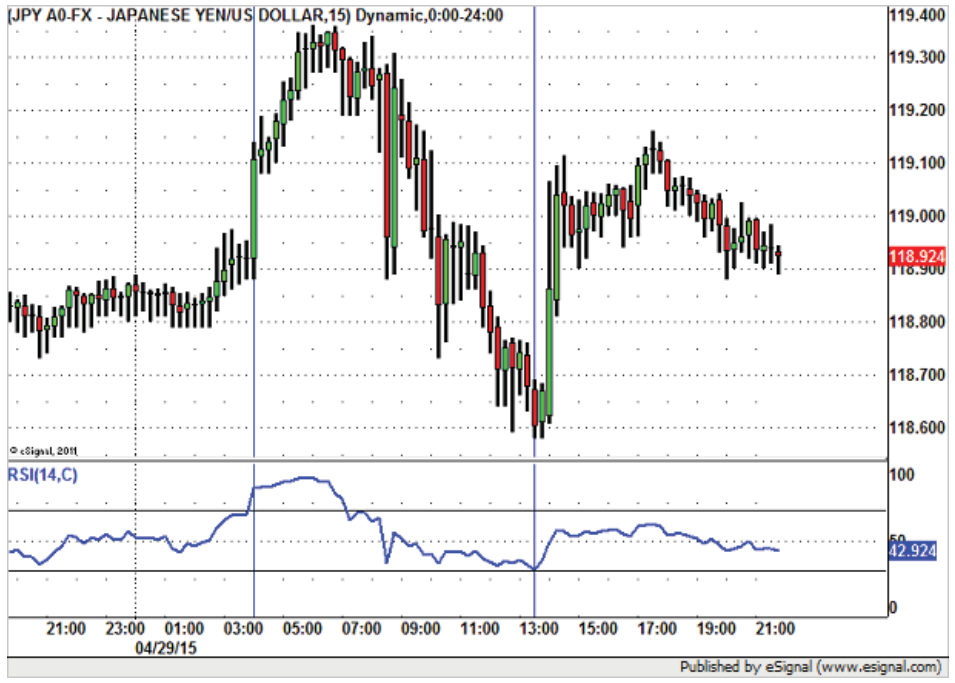
\includegraphics[width=0.7\textwidth]{content/graphics/USDJPY-15_min_chart}
	\caption{USDJPY 15 minute chart by Lien \cite{BOOK:Lien:2016}: \textit{(a)} RSI above 70 at 03:00
	\textit{(b)} RSI at 30 at 13:00}
	\label{fig:related:USDJPY_15min}
\end{figure}

Entering the market at figure \ref{fig:related:USDJPY_15min}.a when the RSI value was above 70 would of seen a market reversal against the entry trade. Waiting until figure \ref{fig:related:USDJPY_15min}.b was the better entry time with the RSI at 30. Although, Kaufman also states that in a study the average amount of RSI values ranges from the 32 to 72 market. He continues, showing that roughly 50 percent of RSI values fall between this range, indicating that the thresholds may need to be widened. Suggestions of 80 to 20 or 85 to 15 are considered extremely strong indicators as they are hard values to sustain. While the example for figure \ref{fig:related:USDJPY_15min} was an ideal scenario, it would be naive to assume this is always the case. Experimenting with threshold ranges to fit this indicator towards the crypto market will be a research point this project looks into.

The MACD is the difference of two EMAs - usually 12 day (short) and 26 day (long) - and another EMA - usually 9 days - that generate trade signals when the lines intersect. Both Harmon \cite{BOOK:Harmon:2014} and Kaufman \cite{BOOK:Kaufman:2013} evaluate the effectiveness of this indicator to be unreliable for trading as it would require the constant fitting of threshold lines to prevent whipsaws\footnote{A volatile price action in which a security swings back and forth in a chaotic pattern}. However, defining thresholds It would seem that this strategy would work well in an upward or downward market interval, but it would result in poor trades in a sideways market due to whipsaws of the trend line intersections. They state that MACDs are ultimately used to define divergence signals.

Utilising both RSI and MACD in this project's trading strategy will indicate if market reversals are likely to occur or if the momentum is still heading in a certain direction. A point Lien \cite{BOOK:Lien:2016} emphasises is the importance of utilising multiple time frames with these indicators as to understand the bigger picture of the market. Failing to analyse where the current moment in the market is can lead to poor trades on the larger scale. Both Kaufman \cite{BOOK:Kaufman:2013} and Harmon also discuss this point in the varying strategies based on multiple time frames. They all conclude to how analysis of multiple time frames can prevent short comings.

The common themes by Kaufman \cite{BOOK:Kaufman:2013}, Harmon \cite{BOOK:Harmon:2014}, Lien \cite{BOOK:Lien:2016}, and Detzel et al \cite{ART:DetzelEtAl:2018} identify valid techniques through


\section{Cryptocurrencies And Their Markets}
\label{sec:related:cryptoAndTheirMarkets}
% Talk about crypto responding to news and biased trading

While low latency millisecond transactions are essential to the stock market, the same methods would fail due to the inadequate latency times and heavy network restrictions set by crypto exchanges. Bloomberg's Levine reports \cite{WEB:Levine:2018} that only recently updates coming from the largest US based crypto exchange - Coinbase\footnote{https://www.coinbase.com/} - are betting on becoming the first to support low latency HFT by offering colocation\footnote{Locating computers owned by trading firms inside the same area as the exchange's servers}. This scarcity of low latency communication between exchange and trader prevents some trading strategies from being applied to the crypto market. The discussion of trading strategies suitable for crypto markets are discussed in section \ref{sec:related:tradingStrategies}.

However, HFT in the crypto market is still apparent despite missing the quoted low latency fundamental that Chorida et al \cite{REPORT:ChordiaEtAl:2013} suggest. Trading is still faster than what any human can achieve and analysis still occurs on the millisecond time frame, but server latency is sub par compared to the stock market. Meyer and Rennison \cite{ART:Meyer:2017} report that large proprietary HFT firms DRW, Jump Trading, DV Trading and Hehmeyer Trading have entered the crypto market. It would be clear to assume that DRW and others have only entered this space if there is profit to be made. This is due to some HFT strategies - such as arbitrage (See section \ref{sec:related:tradingStrategies}) - not requiring transactions to occur on the millisecond time frame. Other types of AT may also be used such as trend lines, technical analysis and market making (See section \ref{sec:related:tradingStrategies}). 

Thus, by using the suggested strategies as examples, or most likely some unreleased strategies that are kept secret, the crypto market has the potential for profit to be made. Furthermore, this suggests that low latency is also not a fundamental requirement for HFT to be successful in crypto markets and the use of other strategies can also be utilised. Literature on algorithms applying technical analysis are sparse, however how technical analysis can be applied towards both markets is discussed in section \ref{sec:related:tradingStrategies}.

% Crpyto is in between currency and securities like stocks, discuss this

\section{Conclusion}
\label{sec:related:conclusion}

